\section{Final Tables}
The summarized results are presented in three tables: 
\begin{itemize}
\item Table~\ref{tab:OSSF1tau0} contains observed yields  and background prediction 
for each search region in a tri-lepton channel with an opposite sign same flavour lepton pair present;
\item Table~\ref{tab:OSSF0tau0}  - for a channel without  an opposite sign same flavour lepton pair;
\item Table~\ref{tab:SStau1} - for a channel with a same sign di-lepton and a hadronically decaying tau (SS$\tau$);
\item Table~\ref{tab:OSOF1tau1} - for a channel with an opposite sign opposite flavour di-lepton and a hadronically decaying tau (OSOF$\tau$). This result is fully based on the Ref.~\cite{AN2012:255}.
\end{itemize}

The graphical representation of the results is shown in Figures~\ref{fig:OSSF1tau0},~\ref{fig:OSSF0tau0},~\ref{fig:SStau1},~\ref{fig:OSOF1tau1}.

%==========================================================================================
\begin{figure}[htp]
\begin{center}
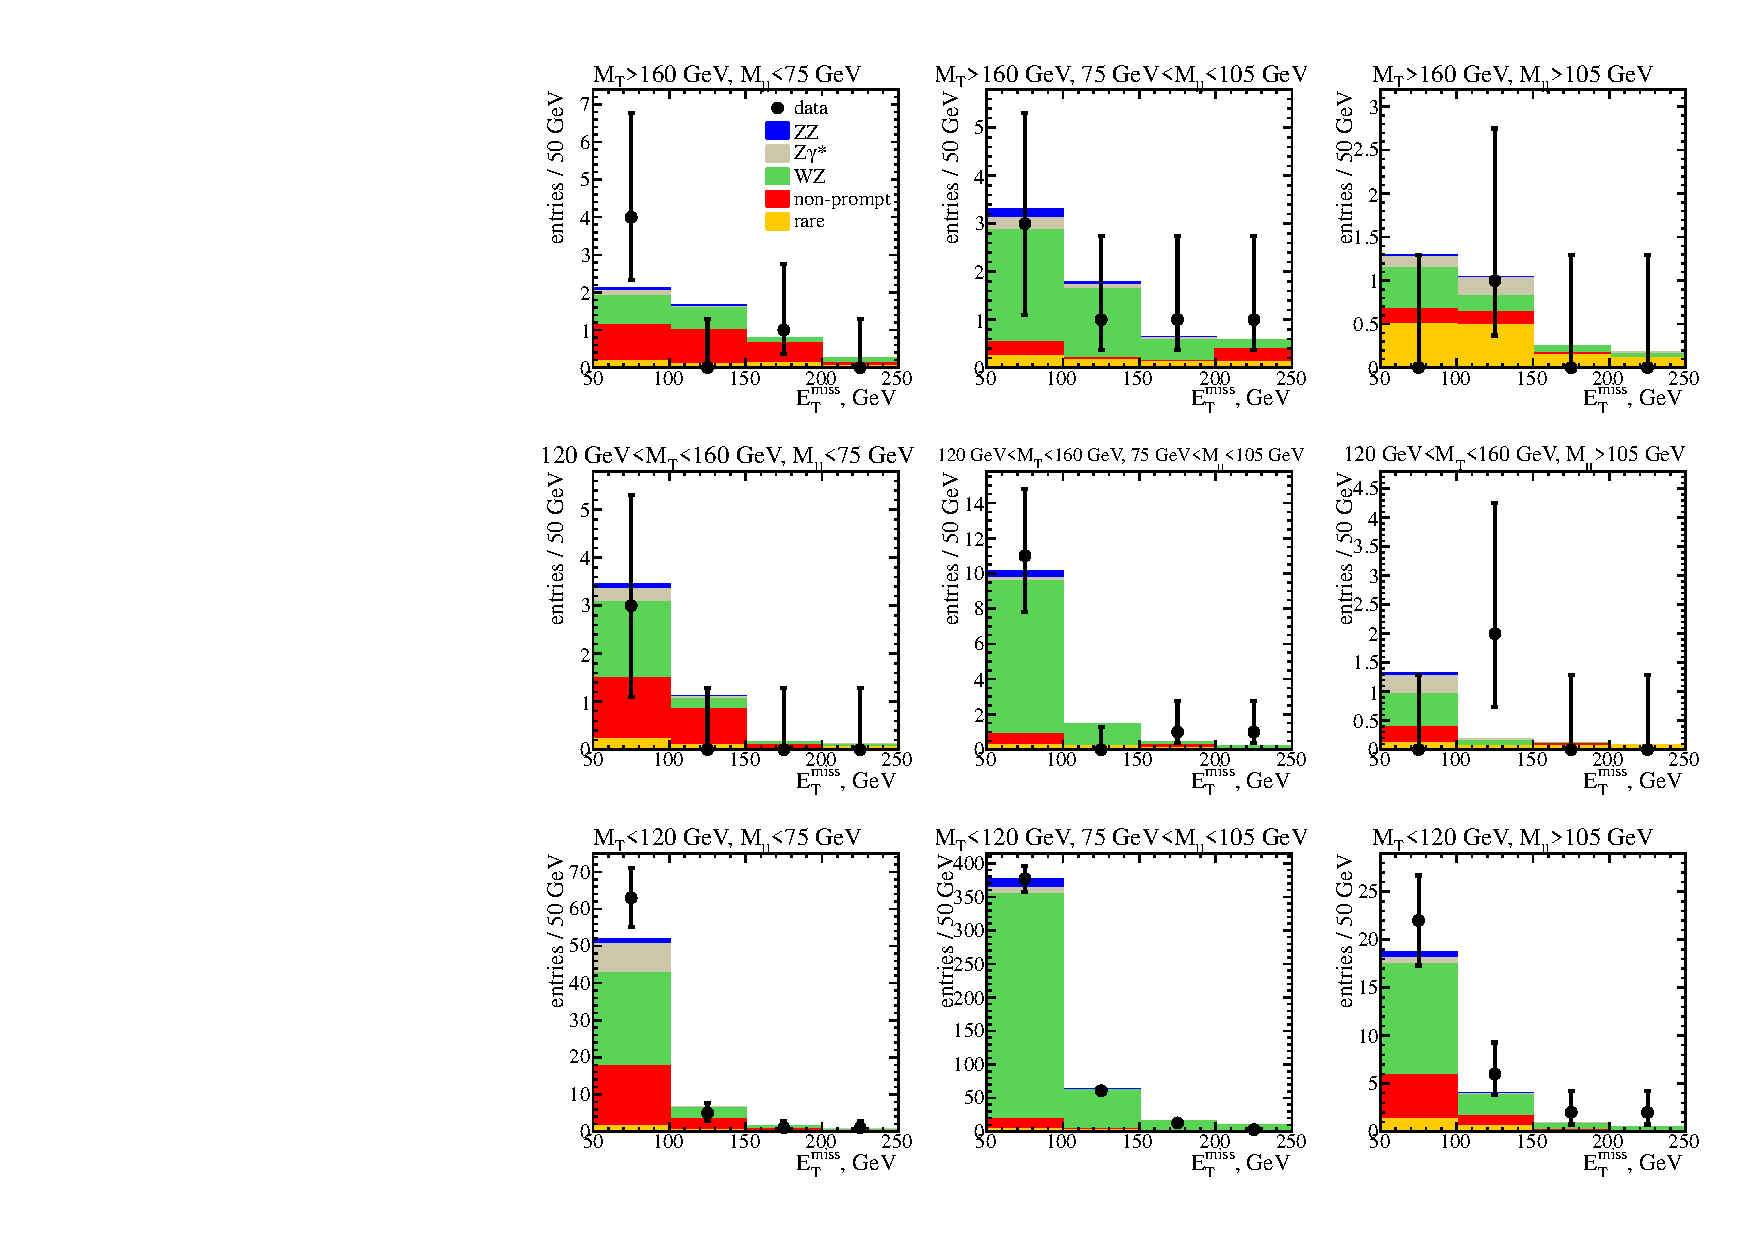
\includegraphics[width=1.0\textwidth]{plots/ossf1tau0.pdf}
\caption{Observed yields and predicted backgrounds for a tri-lepton with an opposite sign same flavour lepton pair present in all defined search regions.}
\label{fig:OSSF1tau0}
\end{center}
\end{figure}
%==========================================================================================

%==========================================================================================
\begin{figure}[htp]
\begin{center}
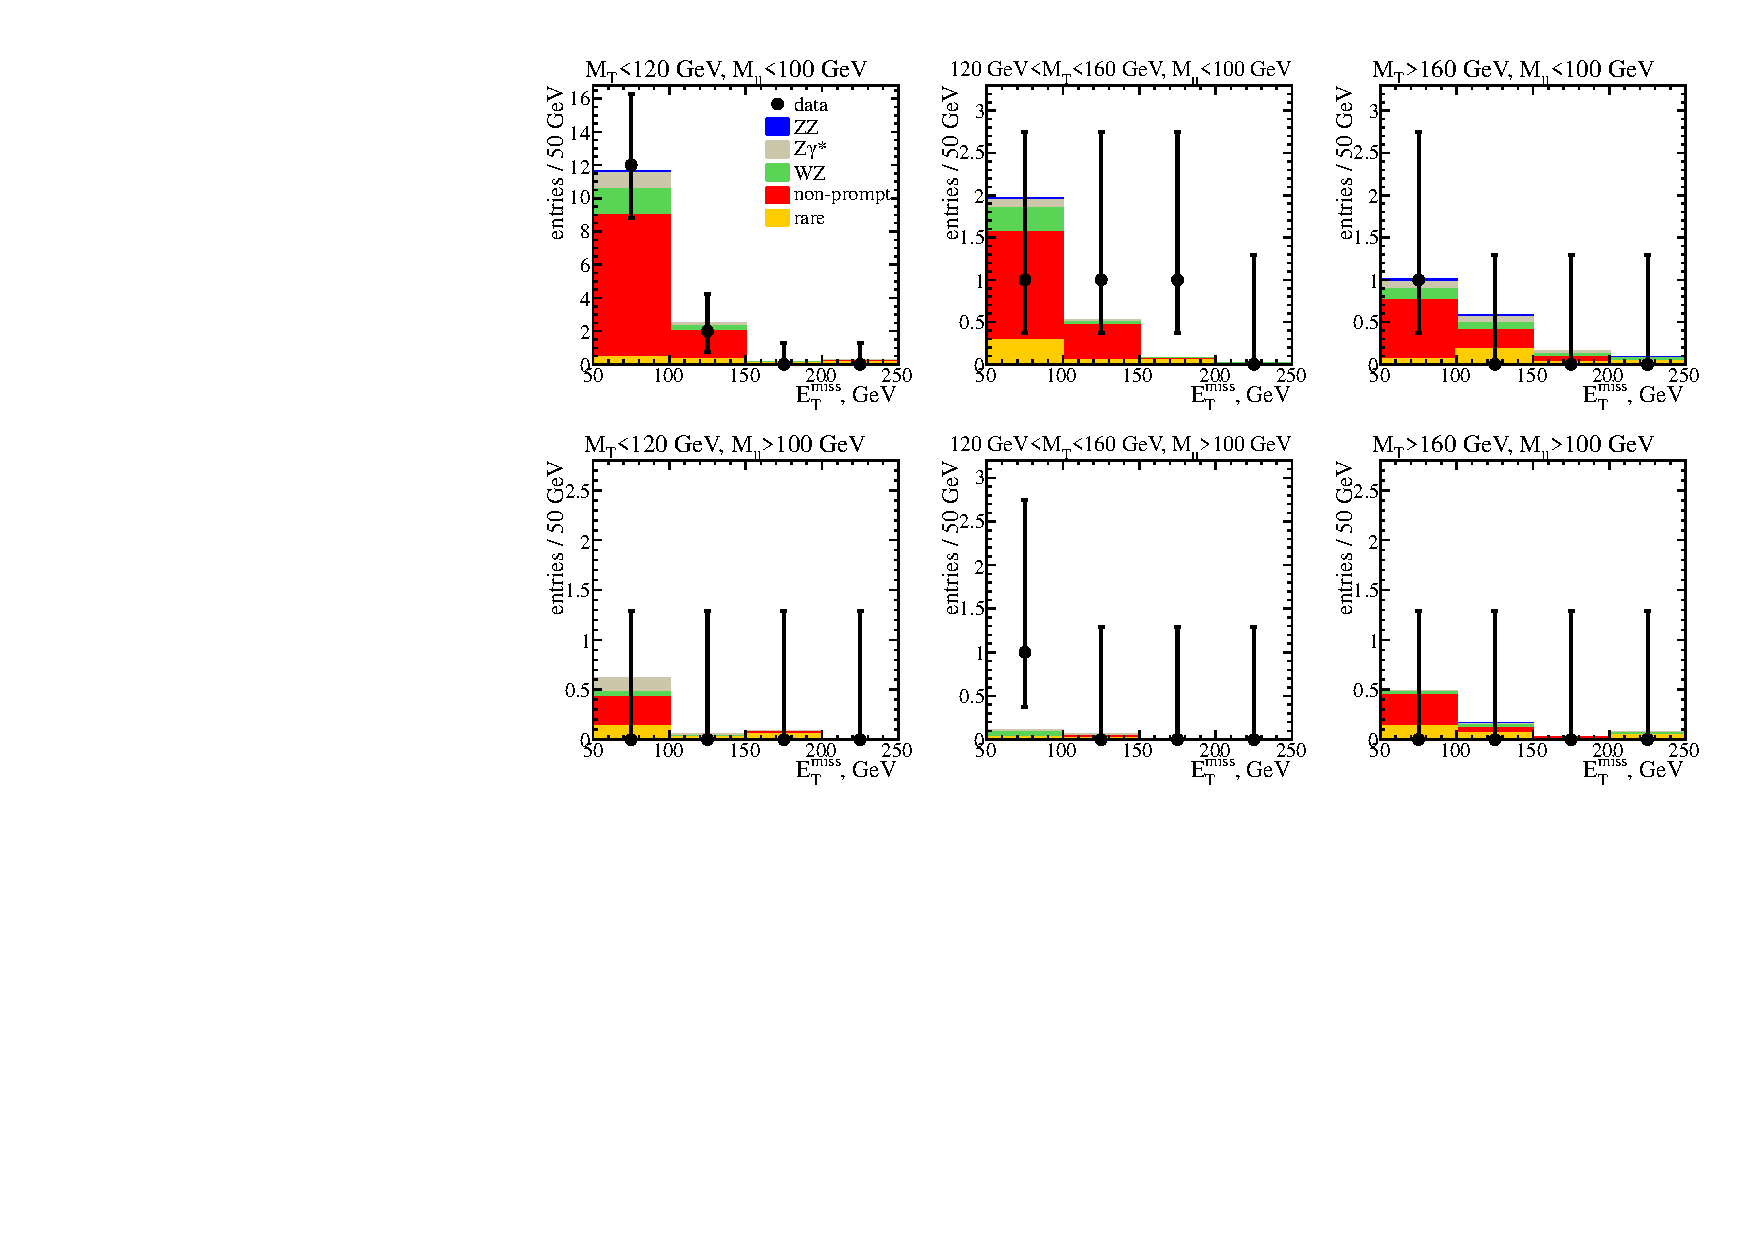
\includegraphics[width=1.0\textwidth]{plots/ossf0tau0.pdf}
\caption{Observed yields and predicted backgrounds for a tri-lepton without an opposite sign same flavour lepton pair present in all defined search regions.}
\label{fig:OSSF0tau0}
\end{center}
\end{figure}
%==========================================================================================

%==========================================================================================
\begin{figure}[htp]
\begin{center}
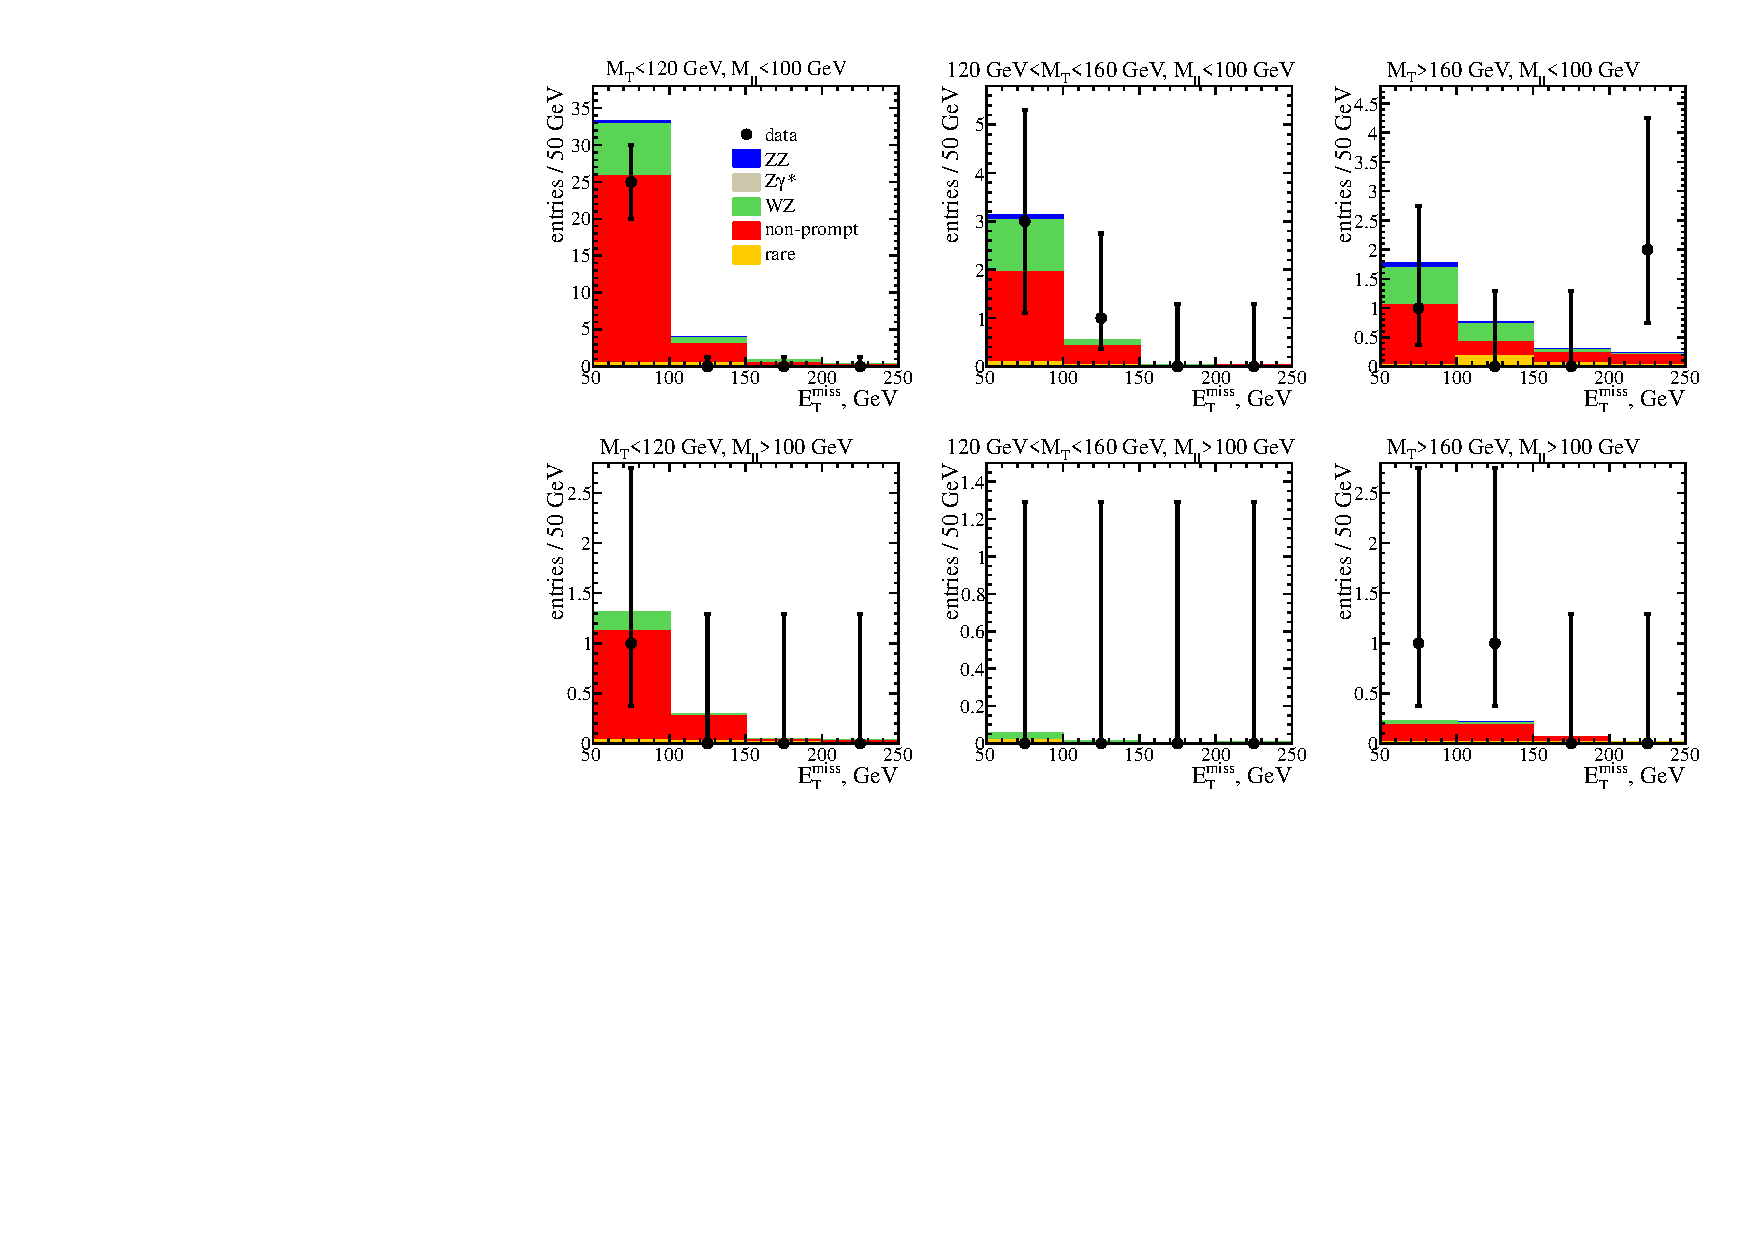
\includegraphics[width=1.0\textwidth]{plots/ossf0tau1.pdf}
\caption{Observed yields and predicted backgrounds for a tri-lepton with a same sign di-lepton and a hadronically decaying tau in all defined search regions.}
\label{fig:SStau1}
\end{center}
\end{figure}
%==========================================================================================

%==========================================================================================
\begin{figure}[htp]
\begin{center}
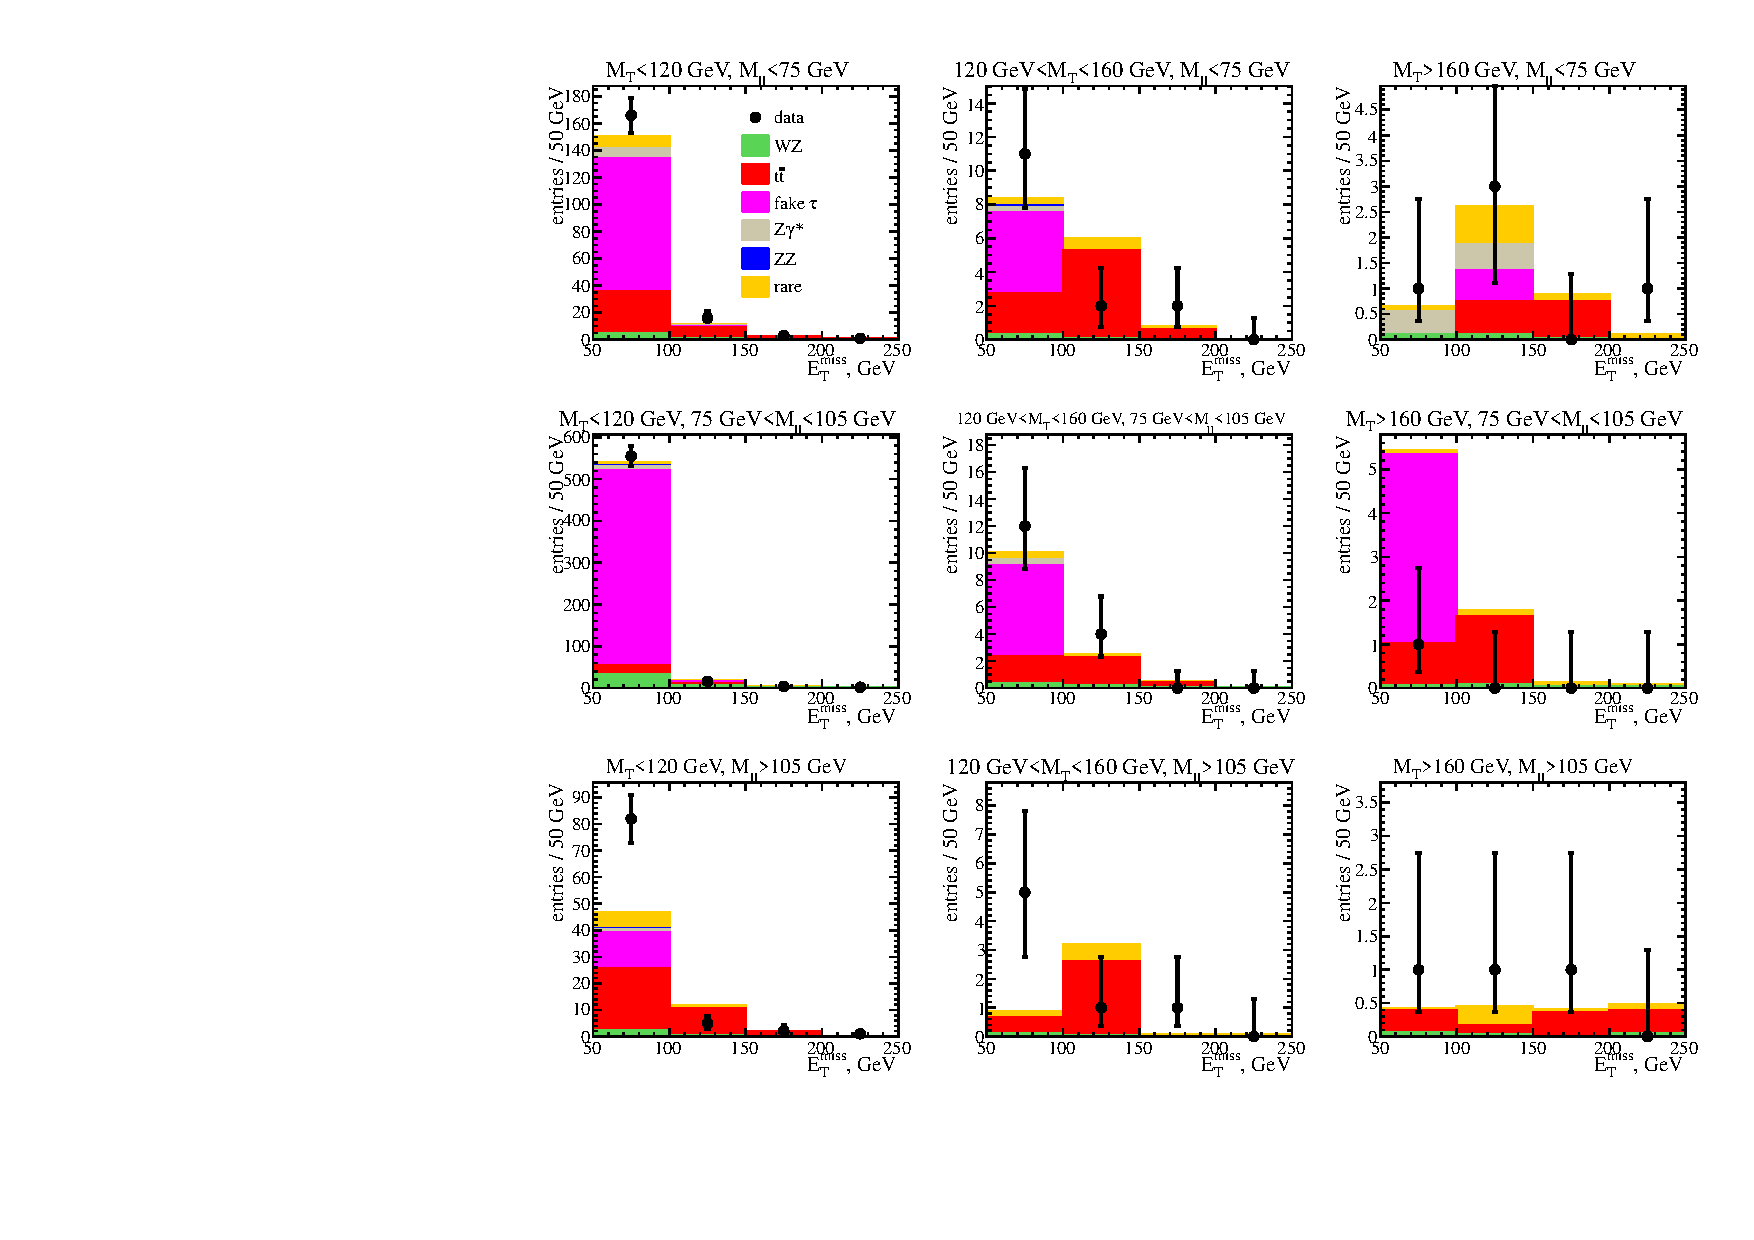
\includegraphics[width=1.0\textwidth]{plots/osof1tau1.pdf}
\caption{Observed yields and predicted backgrounds for a tri-lepton with an opposite sign opposite flavour di-lepton and a hadronically decaying tau  in all defined search regions.}
\label{fig:OSOF1tau1}
\end{center}
\end{figure}
%==========================================================================================

\begin{landscape}
%==========================================================================================
%==========================================================================================
\begin{table}
\begin{center}
\caption{\label{tab:OSSF1tau0} The summary of the observed yields and predicted backgrounds for tri-lepton with opposite sign same flavour pair present. }
\begin{tabular}{| c | c c c c c c c | }\hline\hline
$\ETmiss$ (GeV) & WZ & Non-Prompt & Rare SM & Z$\gamma^*$ & ZZ & Total bkg & Observed\\\hline\hline
\multicolumn{8}{l}{$M_{\text{T}} < 120$ GeV, $M_{\ell\ell} < 75$ GeV}\\\hline\hline
50$\dots$100&27$\pm$2.9&18$\pm$3.5&1.4$\pm$0.84&5.3$\pm$0.24&0.95$\pm$0.02&53$\pm$4.6&63\\
100$\dots$150&3.9$\pm$0.8&2.6$\pm$0.87&0.42$\pm$0.24&0.036$\pm$0.029&0.071$\pm$0.0053&7$\pm$1.2&5\\
150$\dots$200&1.3$\pm$0.53&0.4$\pm$0.21&0.19$\pm$0.13&0$\pm$0.00024&0.014$\pm$0.0023&1.9$\pm$0.59&1\\
200$\dots$250&0.38$\pm$0.12&0.052$\pm$0.05&0.082$\pm$0.058&0$\pm$0.00024&0.004$\pm$0.0011&0.52$\pm$0.14&1\\
\hline\hline
\multicolumn{8}{l}{$M_{\text{T}} < 120$ GeV, $75~\GeV~< M_{\ell\ell} < 105~\GeV~$}\\\hline\hline
50$\dots$100&334$\pm$28&20.6$\pm$3.7&4.1$\pm$2.2&6.47$\pm$0.26&13.20$\pm$0.07&378$\pm$28&378\\
100$\dots$150&62$\pm$9.6&2.9$\pm$0.86&1.8$\pm$1&0.11$\pm$0.038&1.6$\pm$0.025&69$\pm$9.7&61\\
150$\dots$200&17$\pm$3.9&0.34$\pm$0.14&0.64$\pm$0.35&0$\pm$0.0012&0.29$\pm$0.011&18$\pm$3.9&13\\
200$\dots$250&9.4$\pm$1.9&0.03$\pm$0.028&0.55$\pm$0.3&-0.0012$\pm$0.00074&0.11$\pm$0.0053&10$\pm$1.9&3\\
\hline\hline
\multicolumn{8}{l}{$M_{\text{T}} < 120$ GeV, $M_{\ell\ell} > 105$ GeV}\\\hline\hline
50$\dots$100&12$\pm$1.7&4.5$\pm$1.2&1.2$\pm$0.7&0.74$\pm$0.099&0.58$\pm$0.015&19$\pm$2.2&22\\
100$\dots$150&2.4$\pm$0.36&0.95$\pm$0.37&0.53$\pm$0.3&0.12$\pm$0.039&0.086$\pm$0.0059&4.1$\pm$0.61&6\\
150$\dots$200&0.7$\pm$0.18&0.087$\pm$0.062&0.068$\pm$0.041&0.036$\pm$0.019&0.026$\pm$0.0032&0.92$\pm$0.2&2\\
200$\dots$250&0.37$\pm$0.078&0.055$\pm$0.035&0.029$\pm$0.021&-3.9e-05$\pm$0.00036&0.01$\pm$0.0016&0.47$\pm$0.088&2\\
\hline\hline
\multicolumn{8}{l}{$120~\GeV~< M_{\text{T}} < 160~\GeV~$, $M_{\ell\ell} < 75$ GeV}\\\hline\hline
50$\dots$100&1.7$\pm$0.28&1.4$\pm$0.47&0.22$\pm$0.14&0.18$\pm$0.042&0.089$\pm$0.006&3.5$\pm$0.56&3\\
100$\dots$150&0.28$\pm$0.045&0.81$\pm$0.39&0.091$\pm$0.067&0.036$\pm$0.019&0.006$\pm$0.0016&1.2$\pm$0.4&0\\
150$\dots$200&0.073$\pm$0.032&0.08$\pm$0.052&0.015$\pm$0.014&0$\pm$0.00032&0$\pm$0&0.17$\pm$0.063&0\\
200$\dots$250&0.054$\pm$0.027&0$\pm$1.1e-06&0.044$\pm$0.044&0.018$\pm$0.013&0$\pm$0&0.12$\pm$0.053&0\\
\hline\hline
\multicolumn{8}{l}{$120~\GeV~< M_{\text{T}} < 160~\GeV~$, $75~\GeV~< M_{\ell\ell} < 105~\GeV~$}\\\hline\hline
50$\dots$100&8.4$\pm$1.4&0.7$\pm$0.37&0.25$\pm$0.15&0.1$\pm$0.034&0.37$\pm$0.012&9.9$\pm$1.5&11\\
100$\dots$150&1.4$\pm$0.31&5.9e-07$\pm$0.0001&0.17$\pm$0.11&0$\pm$0.00054&0.029$\pm$0.0034&1.6$\pm$0.33&0\\
150$\dots$200&0.22$\pm$0.1&0.22$\pm$0.19&0.071$\pm$0.054&0$\pm$0.00034&0.004$\pm$0.0013&0.52$\pm$0.22&1\\
200$\dots$250&0.12$\pm$0.023&0.029$\pm$0.031&0.014$\pm$0.014&0$\pm$0.00017&0.0012$\pm$0.00057&0.17$\pm$0.041&1\\
\hline\hline
\end{tabular}
\end{center}
\end{table}
%==========================================================================================
%==========================================================================================
\begin{table*}
\begin{center}
%\caption{Continuation}
\begin{tabular}{| c | c c c c c c c | }\hline\hline
$\ETmiss$ (GeV) & WZ & Non-Prompt & Rare SM & Z$\gamma^*$ & ZZ & Total bkg & Observed\\\hline\hline
\multicolumn{8}{l}{$120~\GeV~< M_{\text{T}} < 160~\GeV~$, $M_{\ell\ell} > 105$ GeV}\\\hline\hline
50$\dots$100&0.65$\pm$0.1&0.59$\pm$0.4&0.11$\pm$0.071&0.069$\pm$0.026&0.035$\pm$0.0038&1.4$\pm$0.42&0\\
100$\dots$150&0.09$\pm$0.037&0.12$\pm$0.085&0.055$\pm$0.047&0.018$\pm$0.013&0.002$\pm$0.0009&0.29$\pm$0.1&2\\
150$\dots$200&0.036$\pm$0.013&0.029$\pm$0.031&0.055$\pm$0.049&0$\pm$0.00017&0.0008$\pm$0.00057&0.12$\pm$0.059&0\\
200$\dots$250&0$\pm$0.0034&0$\pm$1.2e-06&0.077$\pm$0.086&0$\pm$0.00022&0$\pm$0&0.077$\pm$0.086&0\\
\hline\hline
\multicolumn{8}{l}{$M_{\text{T}} > 160$ GeV, $M_{\ell\ell} < 75$ GeV}\\\hline\hline
50$\dots$100&0.85$\pm$0.19&1.1$\pm$0.56&0.16$\pm$0.19&0.12$\pm$0.035&0.081$\pm$0.0057&2.3$\pm$0.63&4\\
100$\dots$150&0.6$\pm$0.064&0.74$\pm$0.54&0.096$\pm$0.11&0.043$\pm$0.024&0.039$\pm$0.004&1.5$\pm$0.56&0\\
150$\dots$200&0.18$\pm$0.064&0.74$\pm$0.53&0.11$\pm$0.13&-3.6e-05$\pm$0.0057&0.0088$\pm$0.0019&1$\pm$0.55&1\\
200$\dots$250&0.2$\pm$0.042&0.053$\pm$0.042&0.033$\pm$0.038&-7.2e-05$\pm$0.00025&0.0056$\pm$0.0013&0.3$\pm$0.07&0\\
\hline\hline
\multicolumn{8}{l}{$M_{\text{T}} > 160$ GeV, $75~\GeV~< M_{\ell\ell} < 105~\GeV~$}\\\hline\hline
50$\dots$100&2.5$\pm$0.44&0.28$\pm$0.13&0.24$\pm$0.27&0.13$\pm$0.035&0.14$\pm$0.0074&3.3$\pm$0.54&3\\
100$\dots$150&1.6$\pm$0.15&0.033$\pm$0.034&0.15$\pm$0.17&0.018$\pm$0.013&0.053$\pm$0.0046&1.8$\pm$0.23&1\\
150$\dots$200&0.53$\pm$0.1&0.015$\pm$0.016&0.12$\pm$0.14&-0.00075$\pm$0.00036&0.011$\pm$0.0021&0.68$\pm$0.17&1\\
200$\dots$250&0.22$\pm$0.042&0.47$\pm$0.32&0.11$\pm$0.12&-0.00045$\pm$0.00017&0.006$\pm$0.0013&0.8$\pm$0.35&1\\
\hline\hline
\multicolumn{8}{l}{$M_{\text{T}} > 160$ GeV, $M_{\ell\ell} > 105$ GeV}\\\hline\hline
50$\dots$100&0.45$\pm$0.061&0.2$\pm$0.18&0.5$\pm$0.66&0.018$\pm$0.013&0.022$\pm$0.003&1.2$\pm$0.69&0\\
100$\dots$150&0.21$\pm$0.067&0.081$\pm$0.04&0.49$\pm$0.62&0.13$\pm$0.036&0.012$\pm$0.0022&0.92$\pm$0.62&1\\
150$\dots$200&0.083$\pm$0.016&0.026$\pm$0.023&0.14$\pm$0.17&-0.00092$\pm$0.00041&0.0036$\pm$0.0012&0.25$\pm$0.17&0\\
200$\dots$250&0.068$\pm$0.014&-0.0002$\pm$4.9e-05&0.11$\pm$0.14&-0.0013$\pm$0.00021&0.0016$\pm$0.00069&0.17$\pm$0.14&0\\
\hline\hline
\end{tabular}
\end{center}
\end{table*}
%==========================================================================================
%==========================================================================================
\begin{table}
\small
\begin{center}
\caption{\label{tab:OSSF0tau0} The summary of the observed yields and predicted backgrounds for tri-lepton without opposite sign same flavour pair present. }
\begin{tabular}{| c | c c c c c c c | }\hline\hline
$\ETmiss$ (GeV) & WZ & Non-Prompt & Rare SM & Z$\gamma^*$ & ZZ & Total bkg & Observed\\\hline\hline
\multicolumn{8}{l}{$M_{\text{T}} < 120$ GeV, $M_{\ell\ell} < 100$ GeV}\\\hline\hline
50$\dots$100&1.7$\pm$0.15&9.6$\pm$2.2&0.44$\pm$0.26&0.65$\pm$0.069&0.12$\pm$0.007&13$\pm$2.2&12\\
100$\dots$150&0.42$\pm$0.084&1.8$\pm$0.6&0.29$\pm$0.18&0.12$\pm$0.031&0.0096$\pm$0.002&2.7$\pm$0.63&3\\
150$\dots$200&0.19$\pm$0.074&0.24$\pm$0.12&0.062$\pm$0.05&0.009$\pm$0.0078&0.0024$\pm$0.00098&0.5$\pm$0.15&0\\
200$\dots$250&0.092$\pm$0.027&0.014$\pm$0.0089&0.13$\pm$0.14&-8.4e-05$\pm$0.00014&0.0004$\pm$0.0004&0.24$\pm$0.14&0\\
\hline\hline
\multicolumn{8}{l}{$M_{\text{T}} < 120$ GeV, $M_{\ell\ell} > 100$ GeV}\\\hline\hline
50$\dots$100&0.036$\pm$0.018&0.39$\pm$0.19&0.14$\pm$0.086&0.12$\pm$0.025&0.004$\pm$0.0013&0.68$\pm$0.21&0\\
100$\dots$150&0.017$\pm$0.0057&0.054$\pm$0.035&0.025$\pm$0.019&0$\pm$0.0051&0$\pm$0&0.096$\pm$0.04&0\\
150$\dots$200&0.0046$\pm$0.002&0.029$\pm$0.024&0.056$\pm$0.049&0$\pm$7.7e-05&0.0008$\pm$0.00057&0.09$\pm$0.055&0\\
200$\dots$250&0$\pm$0&-0.00012$\pm$8.7e-05&0.00021$\pm$0.00017&-3.2e-05$\pm$3.1e-05&0$\pm$0&5.2e-05$\pm$0.00019&0\\
\hline\hline
\multicolumn{8}{l}{$120~\GeV~< M_{\text{T}} < 160~\GeV~$, $M_{\ell\ell} < 100$ GeV}\\\hline\hline
50$\dots$100&0.22$\pm$0.023&1.2$\pm$0.49&0.28$\pm$0.22&0.056$\pm$0.02&0.038$\pm$0.0039&1.8$\pm$0.54&1\\
100$\dots$150&0.05$\pm$0.055&0.4$\pm$0.24&0.051$\pm$0.036&0.027$\pm$0.013&0.0012$\pm$0.00069&0.52$\pm$0.25&0\\
150$\dots$200&0.031$\pm$0.011&0.017$\pm$0.018&0.047$\pm$0.046&0$\pm$8.7e-05&0.0008$\pm$0.00057&0.096$\pm$0.05&1\\
200$\dots$250&0.019$\pm$0.018&0.037$\pm$0.038&0.0068$\pm$0.0062&0$\pm$0&0$\pm$0&0.062$\pm$0.042&0\\
\hline\hline
\multicolumn{8}{l}{$120~\GeV~< M_{\text{T}} < 160~\GeV~$, $M_{\ell\ell} > 100$ GeV}\\\hline\hline
50$\dots$100&0.054$\pm$0.0064&0.0041$\pm$0.005&0.023$\pm$0.019&0.0087$\pm$0.0066&0.0012$\pm$0.00069&0.091$\pm$0.021&1\\
100$\dots$150&0.0054$\pm$0.0071&0$\pm$0.00021&0.014$\pm$0.014&0$\pm$0.003&0$\pm$0&0.02$\pm$0.016&0\\
150$\dots$200&0$\pm$0&0$\pm$4.2e-05&0.00021$\pm$0.00018&0$\pm$0&0$\pm$0&0.00021$\pm$0.00019&0\\
200$\dots$250&0$\pm$0&0$\pm$0&0.004$\pm$0.0046&0$\pm$0&0$\pm$0&0.004$\pm$0.0046&0\\
\hline\hline
\multicolumn{8}{l}{$M_{\text{T}} > 160$ GeV, $M_{\ell\ell} < 100$ GeV}\\\hline\hline
50$\dots$100&0.098$\pm$0.02&0.37$\pm$0.26&0.058$\pm$0.068&0.055$\pm$0.02&0.025$\pm$0.0032&0.61$\pm$0.27&1\\
100$\dots$150&0.1$\pm$0.024&0.76$\pm$0.44&0.18$\pm$0.23&0.051$\pm$0.017&0.017$\pm$0.0026&1.1$\pm$0.5&0\\
150$\dots$200&0.065$\pm$0.021&0.064$\pm$0.035&0.022$\pm$0.026&0.014$\pm$0.0097&0.0044$\pm$0.0013&0.17$\pm$0.049&0\\
200$\dots$250&0.081$\pm$0.014&0.024$\pm$0.018&0.039$\pm$0.047&-0.00077$\pm$0.00015&0.0012$\pm$0.00057&0.14$\pm$0.052&0\\
\hline\hline
\multicolumn{8}{l}{$M_{\text{T}} > 160$ GeV, $M_{\ell\ell} > 100$ GeV}\\\hline\hline
50$\dots$100&0.012$\pm$0.0078&0.4$\pm$0.33&0.13$\pm$0.16&0.009$\pm$0.0082&0.002$\pm$0.0009&0.55$\pm$0.37&0\\
100$\dots$150&0.022$\pm$0.0052&0.053$\pm$0.041&0.06$\pm$0.076&0.0089$\pm$0.0066&0.0008$\pm$0.00057&0.15$\pm$0.087&0\\
150$\dots$200&0.0097$\pm$0.0015&0.021$\pm$0.022&0.00061$\pm$0.00073&-0.00023$\pm$0.00013&0.0004$\pm$0.0004&0.032$\pm$0.022&0\\
200$\dots$250&0.027$\pm$0.0025&-8.4e-05$\pm$1.7e-05&0.044$\pm$0.058&-0.00012$\pm$5.9e-05&0$\pm$0&0.071$\pm$0.058&0\\
\hline\hline
\end{tabular}
\end{center}
\end{table}
%==========================================================================================
%==========================================================================================
\begin{table}
\small
\begin{center}
\caption{\label{tab:SStau1} The summary of the observed yields and predicted backgrounds for the channel with a same sign di-lepton and a hadronically decaying tau. }
\begin{tabular}{| c | c c c c c c c | }\hline\hline
$\ETmiss$ (GeV) & WZ & Non-Prompt & Rare SM & Z$\gamma^*$ & ZZ & Total bkg & Observed\\\hline\hline
\multicolumn{8}{l}{$M_{\text{T}} < 120$ GeV, $M_{\ell\ell} < 100$ GeV}\\\hline\hline
50$\dots$100&7.1$\pm$0.19&18$\pm$2.5&0.41$\pm$6.4&0$\pm$0&0.44$\pm$0.013&26$\pm$2.5&25\\
100$\dots$150&0.87$\pm$0.065&1.6$\pm$0.44&0.61$\pm$1&0$\pm$0&0.028$\pm$0.0033&3.1$\pm$0.76&0\\
150$\dots$200&0.4$\pm$0.044&0.58$\pm$0.4&0.032$\pm$0.26&0$\pm$0&0.0024$\pm$0.00098&1$\pm$0.41&0\\
200$\dots$250&0.21$\pm$0.032&0.034$\pm$0.028&0.014$\pm$0.095&0$\pm$0&0.0012$\pm$0.00069&0.26$\pm$0.044&0\\
\hline\hline
\multicolumn{8}{l}{$M_{\text{T}} < 120$ GeV, $M_{\ell\ell} > 100$ GeV}\\\hline\hline
50$\dots$100&0.19$\pm$0.03&1.1$\pm$0.31&0.043$\pm$0.9&0$\pm$0&0.018$\pm$0.0026&1.3$\pm$0.31&1\\
100$\dots$150&0.026$\pm$0.011&0.12$\pm$0.054&0.013$\pm$0.26&0$\pm$0&0.0024$\pm$0.00098&0.16$\pm$0.058&0\\
150$\dots$200&0.011$\pm$0.0074&0.011$\pm$0.012&0.0096$\pm$0.14&0$\pm$0&0.0012$\pm$0.00069&0.033$\pm$0.017&0\\
200$\dots$250&0.0047$\pm$0.0048&0.0098$\pm$0.012&0.00013$\pm$0.057&0$\pm$0&0.0004$\pm$0&0.015$\pm$0.013&0\\
\hline\hline
\multicolumn{8}{l}{$120~\GeV~< M_{\text{T}} < 160~\GeV~$, $M_{\ell\ell} < 100$ GeV}\\\hline\hline
50$\dots$100&1.1$\pm$0.073&2$\pm$0.6&0.062$\pm$1&0$\pm$0&0.1$\pm$0.0065&3.2$\pm$0.6&3\\
100$\dots$150&0.12$\pm$0.024&0.78$\pm$0.42&0.018$\pm$0.32&0$\pm$0&0.0067$\pm$0.0016&0.92$\pm$0.42&1\\
150$\dots$200&0.02$\pm$0.0098&0$\pm$0&0.0093$\pm$0.029&0$\pm$0&0$\pm$0&0.029$\pm$0.015&0\\
200$\dots$250&0.0055$\pm$0.0052&0.011$\pm$0.012&0.0042$\pm$0.0065&0$\pm$0&0.00039$\pm$0.00039&0.021$\pm$0.013&0\\
\hline\hline
\multicolumn{8}{l}{$120~\GeV~< M_{\text{T}} < 160~\GeV~$, $M_{\ell\ell} > 100$ GeV}\\\hline\hline
50$\dots$100&0.035$\pm$0.013&0$\pm$6.9e-05&0.022$\pm$0.6&0$\pm$0&0.0036$\pm$0.0012&0.061$\pm$0.024&0\\
100$\dots$150&0.013$\pm$0.008&0$\pm$0.0013&0.00018$\pm$0.092&0$\pm$0&0$\pm$0&0.013$\pm$0.0081&0\\
150$\dots$200&0$\pm$0&0$\pm$0&0$\pm$8.6e-05&0$\pm$0&0$\pm$0&0$\pm$0&0\\
200$\dots$250&0.0065$\pm$0.0056&0$\pm$0&0$\pm$0.056&0$\pm$0&0$\pm$0&0.0065$\pm$0.0056&0\\
\hline\hline
\multicolumn{8}{l}{$M_{\text{T}} > 160$ GeV, $M_{\ell\ell} < 100$ GeV}\\\hline\hline
50$\dots$100&0.62$\pm$0.055&0.84$\pm$0.31&0.035$\pm$0.92&0$\pm$0&0.1$\pm$0.0064&1.6$\pm$0.32&1\\
100$\dots$150&0.31$\pm$0.039&0.7$\pm$0.41&0.16$\pm$0.96&0$\pm$0&0.046$\pm$0.0043&1.2$\pm$0.43&0\\
150$\dots$200&0.062$\pm$0.017&0.29$\pm$0.22&0.058$\pm$0.18&0$\pm$0&0.011$\pm$0.0021&0.42$\pm$0.22&0\\
200$\dots$250&0.03$\pm$0.012&0.08$\pm$0.059&0.028$\pm$0.17&0$\pm$0&0.0016$\pm$0.0004&0.14$\pm$0.065&2\\
\hline\hline
\multicolumn{8}{l}{$M_{\text{T}} > 160$ GeV, $M_{\ell\ell} > 100$ GeV}\\\hline\hline
50$\dots$100&0.035$\pm$0.013&0.089$\pm$0.062&0.0052$\pm$0.32&0$\pm$0&0.0028$\pm$0.0011&0.13$\pm$0.064&1\\
100$\dots$150&0.026$\pm$0.011&0.085$\pm$0.074&0.0073$\pm$0.88&0$\pm$0&0.0016$\pm$0.0008&0.12$\pm$0.075&1\\
150$\dots$200&0$\pm$0&0.026$\pm$0.021&0.013$\pm$0.073&0$\pm$0&0.0004$\pm$0.0004&0.04$\pm$0.025&0\\
200$\dots$250&0$\pm$0&-0.00019$\pm$0&0.013$\pm$0.013&0$\pm$0&0.0004$\pm$0.0004&0.013$\pm$0.0097&0\\
\hline\hline
\end{tabular}
\end{center}
\end{table}
%==========================================================================================
%==========================================================================================
\begin{table}
\begin{center}
\caption{\label{tab:OSOF1tau1} The summary of the observed yields and predicted backgrounds for the channel with an OSOF di-lepton and a hadronically decaying tau. }
\begin{tabular}{| c | c c c c c c  | c  c | }\hline\hline
$\ETmiss$ (GeV) & WZ & $t\bar{t}$ & Fake tau & Z$\gamma^*$ & ZZ & Rare SM & Total bkg & Observed\\\hline\hline
\multicolumn{7}{l}{$M_{\text{T}} < 120$ GeV, $M_{\ell\ell} < 75$ GeV}\\\hline\hline
50$\dots$100&4.3$\pm$1.2&12$\pm$6.7&99.7$\pm$49.6&6.9$\pm$3.4&0.7$\pm$0.51&7.6$\pm$4.2&131$\pm$54.7&136\\
100$\dots$150&0.76$\pm$0.23&6.1$\pm$3.6&0.92$\pm$0.82&0.44$\pm$0.48&0$\pm$0&1.3$\pm$0.71&9.4$\pm$4.1&5\\
150$\dots$200&0.21$\pm$0.07&1.2$\pm$0.9&0$\pm$0&0$\pm$0&0$\pm$0&0.076$\pm$0.056&1.5$\pm$0.92&1\\
200$\dots$250&0.098$\pm$0.038&1.4$\pm$1.1&0$\pm$0&0$\pm$0&0$\pm$0&0.011$\pm$0.0087&1.5$\pm$1.1&1\\
\hline\hline
\multicolumn{7}{l}{$M_{\text{T}} < 120$ GeV, $75~\mathrm{GeV} < M_{\ell\ell} < 105~\mathrm{GeV}$}\\\hline\hline
50$\dots$100&30$\pm$8.6&8.9$\pm$5.2&449$\pm$136&8.8$\pm$4.4&3.2$\pm$1.8&8.2$\pm$4.4&508$\pm$145&516\\
100$\dots$150&7$\pm$2&2.5$\pm$1.7&2.6$\pm$1.8&0$\pm$0&0.6$\pm$0.45&0.91$\pm$0.51&14$\pm$4&11\\
150$\dots$200&2.4$\pm$0.68&0$\pm$0&0$\pm$0&0$\pm$0&0$\pm$0&0.17$\pm$0.099&2.5$\pm$0.71&2\\
200$\dots$250&1.3$\pm$0.37&0$\pm$0&0$\pm$0&0$\pm$0&0$\pm$0&0.097$\pm$0.057&1.4$\pm$0.39&1\\
\hline\hline
\multicolumn{7}{l}{$M_{\text{T}} < 120$ GeV, $M_{\ell\ell} > 105$ GeV}\\\hline\hline
50$\dots$100&2.2$\pm$0.65&11$\pm$6.1&14$\pm$5.4&1.2$\pm$0.77&0.28$\pm$0.26&5.9$\pm$3.2&34$\pm$11&57\\
100$\dots$150&0.44$\pm$0.13&4.6$\pm$2.8&0.61$\pm$0.63&0$\pm$0&0$\pm$0&1.3$\pm$0.85&6.9$\pm$3.2&2\\
150$\dots$200&0.11$\pm$0.039&0.75$\pm$0.64&0$\pm$0&0$\pm$0&0$\pm$0&0.095$\pm$0.073&0.95$\pm$0.66&1\\
200$\dots$250&0.061$\pm$0.026&0$\pm$0&0$\pm$0&0$\pm$0&0$\pm$0&0.065$\pm$0.046&0.13$\pm$0.056&0\\
\hline\hline
\multicolumn{7}{l}{$120~\mathrm{GeV} < M_{\text{T}} < 160~\mathrm{GeV}$, $M_{\ell\ell} < 75$ GeV}\\\hline\hline
50$\dots$100&0.29$\pm$0.11&1.7$\pm$1.3&4.8$\pm$3.3&0.31$\pm$0.36&0.21$\pm$0.25&0.42$\pm$0.27&7.8$\pm$4.1&8\\
100$\dots$150&0.047$\pm$0.023&2.2$\pm$1.6&0$\pm$0&0$\pm$0&0$\pm$0&0.69$\pm$0.54&3$\pm$1.8&1\\
150$\dots$200&0.038$\pm$0.022&0.27$\pm$0.32&0$\pm$0&0$\pm$0&0$\pm$0&0.15$\pm$0.12&0.46$\pm$0.35&1\\
200$\dots$250&0.0057$\pm$0.006&0$\pm$0&0$\pm$0&0$\pm$0&0$\pm$0&0.022$\pm$0.024&0.027$\pm$0.025&0\\
\hline\hline
\multicolumn{7}{l}{$120~\mathrm{GeV} < M_{\text{T}} < 160~\mathrm{GeV}$, $75~\mathrm{GeV} < M_{\ell\ell} < 105~\mathrm{GeV}$}\\\hline\hline
50$\dots$100&0.34$\pm$0.13&0.79$\pm$0.69&8.7$\pm$4.3&0.44$\pm$0.45&0$\pm$0&0.51$\pm$0.33&11$\pm$4.8&9\\
100$\dots$150&0.18$\pm$0.072&1$\pm$0.84&0$\pm$0&0$\pm$0&0$\pm$0&0.19$\pm$0.12&1.4$\pm$0.9&3\\
150$\dots$200&0.094$\pm$0.041&0$\pm$0&0$\pm$0&0$\pm$0&0$\pm$0&0.042$\pm$0.027&0.14$\pm$0.056&0\\
200$\dots$250&0.027$\pm$0.016&0$\pm$0&0$\pm$0&0$\pm$0&0$\pm$0&0.052$\pm$0.043&0.079$\pm$0.048&0\\
\hline\hline
\end{tabular}
\end{center}
\end{table}
%==========================================================================================
\begin{table*}
\begin{center}
\begin{tabular}{| c | c c c c c c  | c  c | }\hline\hline
$\ETmiss$ (GeV) & WZ & $t\bar{t}$ & Fake tau & Z$\gamma^*$ & ZZ & Rare SM & Total bkg & Observed\\\hline\hline
\multicolumn{7}{l}{$120~\mathrm{GeV} < M_{\text{T}} < 160~\mathrm{GeV}$, $M_{\ell\ell} > 105$ GeV}\\\hline\hline
50$\dots$100&0.12$\pm$0.052&0.16$\pm$0.19&0$\pm$0&0$\pm$0&0$\pm$0&0.24$\pm$0.16&0.52$\pm$0.28&3\\
100$\dots$150&0.052$\pm$0.025&1.3$\pm$1&0$\pm$0&0$\pm$0&0$\pm$0&0.6$\pm$0.39&2$\pm$1.2&0\\
150$\dots$200&0.0087$\pm$0.0069&0$\pm$0&0$\pm$0&0$\pm$0&0$\pm$0&0.08$\pm$0.066&0.089$\pm$0.068&0\\
200$\dots$250&0.01$\pm$0.011&0$\pm$0&0$\pm$0&0$\pm$0&0$\pm$0&0.00012$\pm$0.00014&0.01$\pm$0.011&0\\
\hline\hline
\multicolumn{7}{l}{$M_{\text{T}} > 160$ GeV, $M_{\ell\ell} < 75$ GeV}\\\hline\hline
50$\dots$100&0.1$\pm$0.11&0$\pm$0&0$\pm$0&0.44$\pm$0.65&0$\pm$0&0.089$\pm$0.11&0.63$\pm$0.8&1\\
100$\dots$150&0.11$\pm$0.12&0$\pm$0&0.61$\pm$0.9&0.51$\pm$0.74&0$\pm$0&0.75$\pm$0.92&2$\pm$2.2&2\\
150$\dots$200&0.019$\pm$0.022&0$\pm$0&0$\pm$0&0$\pm$0&0$\pm$0&0.12$\pm$0.14&0.14$\pm$0.16&0\\
200$\dots$250&0.016$\pm$0.019&0$\pm$0&0$\pm$0&0$\pm$0&0$\pm$0&0.097$\pm$0.12&0.11$\pm$0.13&1\\
\hline\hline
\multicolumn{7}{l}{$M_{\text{T}} > 160$ GeV, $75~\mathrm{GeV} < M_{\ell\ell} < 105~\mathrm{GeV}$}\\\hline\hline
50$\dots$100&0.05$\pm$0.054&0.34$\pm$0.5&4.3$\pm$4.8&0.00044$\pm$0.00064&0$\pm$0&0.092$\pm$0.11&4.8$\pm$5.2&1\\
100$\dots$150&0.086$\pm$0.09&0.84$\pm$1.1&0$\pm$0&0$\pm$0&0$\pm$0&0.13$\pm$0.15&1.1$\pm$1.3&0\\
150$\dots$200&0.043$\pm$0.047&0$\pm$0&0$\pm$0&0$\pm$0&0$\pm$0&0.084$\pm$0.1&0.13$\pm$0.14&0\\
200$\dots$250&0.033$\pm$0.036&0$\pm$0&0$\pm$0&0$\pm$0&0$\pm$0&0.053$\pm$0.061&0.085$\pm$0.092&0\\
\hline\hline
\multicolumn{7}{l}{$M_{\text{T}} > 160$ GeV, $M_{\ell\ell} > 105$ GeV}\\\hline\hline
50$\dots$100&0.062$\pm$0.066&0.32$\pm$0.48&0$\pm$0&0$\pm$0&0$\pm$0&0.032$\pm$0.049&0.42$\pm$0.55&0\\
100$\dots$150&0.041$\pm$0.044&0.11$\pm$0.17&0$\pm$0&0$\pm$0&0$\pm$0&0.2$\pm$0.24&0.35$\pm$0.4&0\\
150$\dots$200&0.0096$\pm$0.012&0$\pm$0&0$\pm$0&0$\pm$0&0$\pm$0&0.047$\pm$0.066&0.057$\pm$0.074&0\\
200$\dots$250&0.041$\pm$0.046&0$\pm$0&0$\pm$0&0$\pm$0&0$\pm$0&0.091$\pm$0.11&0.13$\pm$0.15&0\\
\hline\hline
\end{tabular}
\end{center}
\end{table*}
%==========================================================================================
%==========================================================================================
\end{landscape}